\chapter{El LHC y el detector ATLAS}
\label{cap:detector}

%% Para explorar la región de energías del {\tev}, en el laboratorio CERN se construyó
%% el Gran Colisionador de Hadrones,
%% diseñado para colisionar protones a una energía de centro de masa de $\sqrt{s} = 14 \tev$.


%% Uno de los detectores multipropósito del LHC es ATLAS.

%% En este capítulo se realiza una breve descripción del LHC y en particular
%% del detector ATLAS.


\section{LHC}

El Gran Colisionador de Hadrones (LHC, del inglés \emph{Large Hadron Collider})
\cite{Evans:1129806} es el acelerador de hadrones del Centro Europeo para la
Investigación Nuclear (CERN), ubicado en la frontera entre Francia y Suiza.
Posee una longitud de 27 km y fue construido en el mismo túnel en el que
funcionaba el acelerador $e^{+}e^{-}$ LEP \cite{LEP} (entre 1989 y 2000), a una
profundidad variable entre 50 y 174 m de la superficie.

El complejo de aceleradores del CERN (ver \cref{fig:lhc_complex}) es una
sucesión de aceleradores, en la cual cada acelerador inyecta el haz de protones
en el siguiente, que se encarga de elevar la energía un poco más. El LHC, que es
el último elemento en la cadena, está diseñado para acelerar cada haz de
protones a 7 \tev, alcanzando en las colisiones, energías de centro de masa de
14 \tev, y una luminosidad de $10^{34}$ cm$^{-2}$s$^{-1}$. Los demás
aceleradores en la cadena poseen además otros experimentos que utilizan los
haces a menores energías.

El número de eventos producidos en un colisionador, como el LHC, está dado
por:

\begin{equation}
  N = L \, \sigma
\end{equation}
%
donde $\sigma$ es la sección eficaz del proceso físico y $L$ es la luminosidad instantánea del
acelerador.

%% La luminosidad instantanea se define como el número de protones que pasan por unidad
%% de area y unidad de tiempo.

La luminosidad instantánea es uno de los parámetros más importantes para
caracterizar el funcionamiento del acelerador, definida como el número de
partículas (protones o iones pesados en el caso del LHC) por unidad de tiempo y unidad de
área, y puede calcularse mediante la relación:

\begin{equation}
  L = f_\text{rev} n_b \frac{N_1 N_2}{A}
\end{equation}
%
donde $f_\text{rev}$ es la frecuencia de revolución ($\sim 11$ kHz), $n_b$ es el número de
\emph{bunches} (paquetes de protones) por haz, $N_i$ es el número de partículas
en cada \emph{bunch} y $A$ es la sección efectiva del haz, que puede expresarse en
término de los parámetros del acelerador como:

\begin{equation}
  A = \frac{4\pi \epsilon_n \beta^{*}}{\gamma F}
\end{equation}
%
donde $\epsilon_n$ es la emitancia transversal normalizada (la dispersión
transversal media de las partículas del haz en el espacio de coordenadas e
impulsos), $\beta^{*}$ es la función de amplitud en el punto de interacción,
relacionada al poder de focalización de los cuadrupolos), $\gamma$ es el
factor relativista de Lorentz y $F$ es un factor de reducción geométrico, debido
al ángulo de cruce de los haces en el punto de interacción.

\begin{figure}[!p]
  \centering

  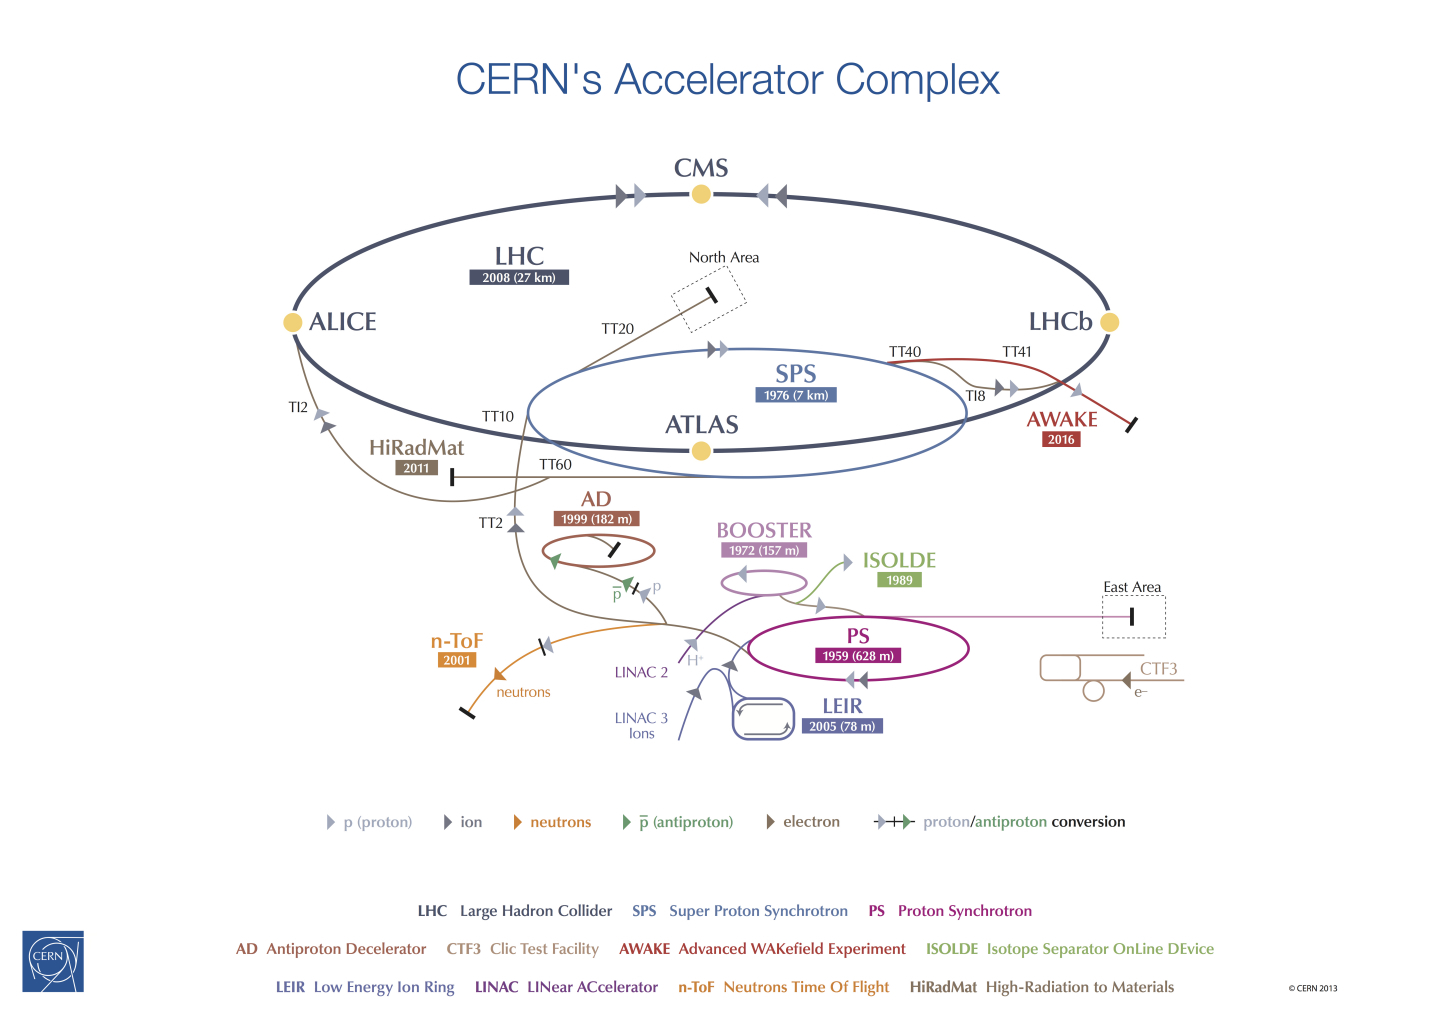
\includegraphics[width=0.9\textwidth]{lhc_complex}

  \caption{Complejo de aceleradores del CERN, incluyendo al LHC y a la serie
    de aceleradores utilizados para proveer de protones al LHC. También pueden verse
    los diferentes experimentos ubicados en el acelerador.}
  \label{fig:lhc_complex}

\end{figure}

El diseño del LHC contempla trenes de 2808 paquetes de $\sim 10^{11}$ protones cada uno,
espaciados temporalmente en $\unit[25]{ns}$.
Para acelerar los haces de protones y mantenerlos en sus órbitas circulares el
LHC cuenta con 1232 dipolos magnéticos superconductores que generan un campo
magnético de $\unit[8.4]{T}$ enfriados a $\unit[1.9]{K}$. El sistema de focalización de los haces
consiste de 392 cuadrupolos magnéticos que generan campos magnéticos de $\unit[6.8]{T}$.
Los haces circulan en direcciones opuestas en cavidades de ultra alto vacío
a presión de $\unit[10^{-10}]{torr}$.

Durante el año 2012, las colisiones se realizaron a $4\TeV$ por haz ($\sqrt{s} = 8 \TeV$)
y con una luminosidad que fue incrementándose hasta alcanzar los
$\unit[2 \cdot 10^{32}]{cm^{-2}s^{-1}}$ en Octubre. Durante los a\~nos 2013 y 2014
el LHC no estuvo en funcionamiento, y se utilizó este tiempo para prepararlo para
la nueva etapa que comenzó en el a\~no 2015, en el cual se alcanzó una energía de $\sqrt{s} = 13 \tev$,
una energía que nunca antes había sido alcanzada y cercana a la de su diseño
original (14 \tev).



\section{El detector ATLAS}

ATLAS (\emph{A Torodial LHC AparatuS}) es un detector de partículas
multipropósito del LHC, diseñado y construido para estudiar las colisiones
protón-protón (y de iones pesados) y un gran espectro de procesos físicos en la
escala de energía del \tev.

\begin{figure}[!p]
  \centering

  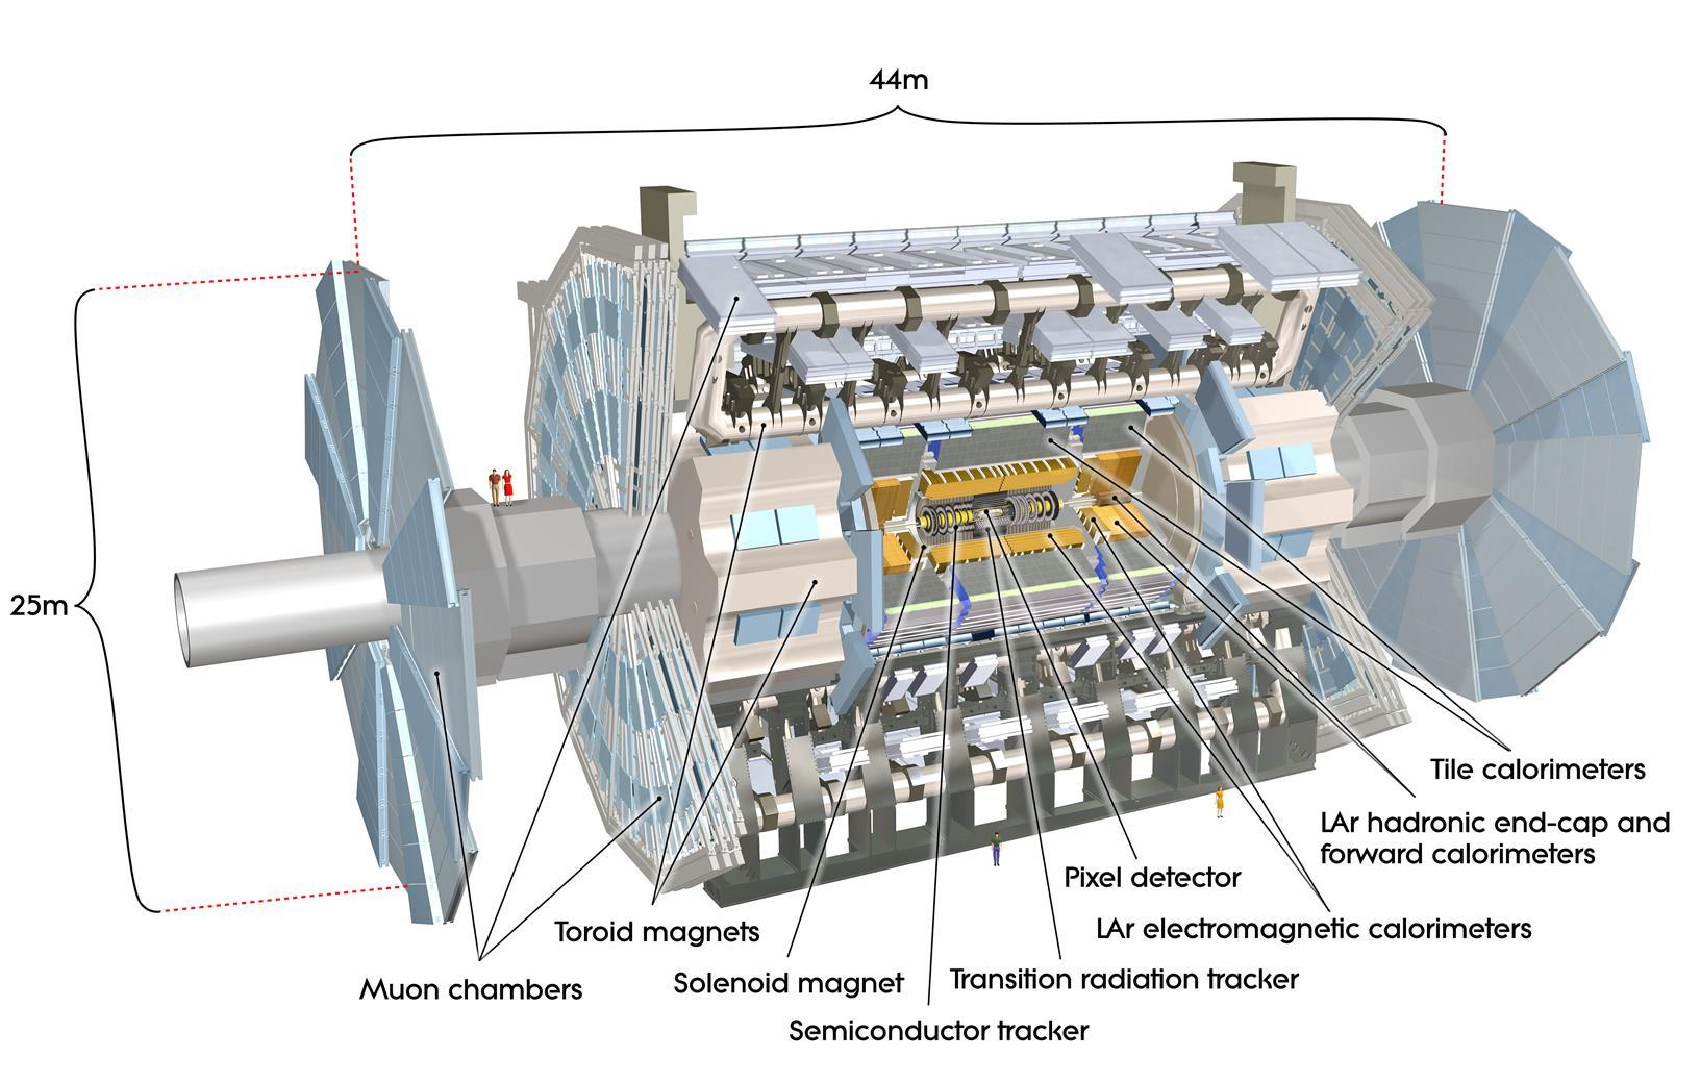
\includegraphics[width=\textwidth]{atlas}
  \caption{Esquema general del detector de ATLAS. Las dimensiones del detector
    son $\unit[25]{m}$ de altura y $\unit[44]{m}$ de largo. El peso promedio es
    de aproximadamente 7000 toneladas.}
  \label{fig:atlas}

\end{figure}

El esquema general del detector se muestra en la \cref{fig:atlas}, donde se
señalan los componentes principales. ATLAS está diseñado en capas de
subdetectores que cumplen diferentes roles en la identificación de las
partículas producidas durante las colisiones (ver \cref{fig:how_atlas_works}).
Desde el punto de la colisión
hacia afuera ATLAS se compone de un detector interno de trazas (ID) compuesto de
un detector de píxeles, un detector de bandas de silicio (SCT) y un detector de
radiación de transición (TRT).
Por sobre el detector interno se encuentra un
solenoide superconductor que genera un campo magnético de $\sim \unit[2]{T}$, a fin
de curvar la trayectoria de las partículas cargadas.
A continuación están ubicados los calorímetros. En primer lugar el calorímetro
electromagnético para medir la energía cinética de electrones y fotones, y
posteriormente el calorímetro hadrónico para medir la energía de los jets.
En la capa más externa se encuentra el espectrómetro de muones que le da a ATLAS
el tamaño total de aproximadamente $\unit[45]{m}$ de largo y más de
$\unit[25]{m}$ de alto. Intercalado con éste se encuentra el sistema de toroides
que genera el campo magnético de $\sim \unit[4]{T}$ para curvar la trayectoria de
los muones hacia el final de su pasaje por el detector ATLAS.

El detector ATLAS se divide geométricamente en dos regiones, la parte central
denominada \emph{barrel}, y la región de las tapas llamadas \emph{end-caps}.
En cada una de estas regiones la ubicación de los
subdetectores es distinta. En la región \emph{barrel}, los subdetectores están
ubicadas como cilindros concéntricos, mientras que en la región \emph{end-cap}
están ubicados como discos consecutivos perpendiculares a la dirección del haz.


\begin{figure}[!p]
  \centering

  \includegraphics[width=0.8\textwidth]{how_atlas_works_invert}

  \caption{Esquema del corte transversal del detector de ATLAS, ilustrando los distintos
  subdetectores y el pasaje de las distintas partículas.}
  \label{fig:how_atlas_works}

\end{figure}


\subsection{Sistema de coordenadas}

%% El sistema de coordenadas de ATLAS corresponde a un sistema cartesiano, cuyo
%% origen coincide con el punto de interacción nominal. El eje $z$ es escogido,
%% naturalmente dazda la concepción cilíndrica del detector, a lo largo del eje del
%% haz, en sentido antihorario.

El sistema de coordenadas y la nomenclatura utilizada para describir el detector
ATLAS y las trayectorias de las partículas que emergen de las colisiones son
resumidas en esta sección, ya que se utilizarán a lo largo de la tesis. Se
define como origen de coordenadas al punto de interacción nominal, mientras que
la dirección del haz define el eje $z$ y el plano $x-y$ es el transversal a la
dirección del haz. El eje $x$ se define desde el punto de interacción, apuntando
al centro del anillo del LHC, y el eje $y$ se define apuntando hacia arriba.

%% El plano transversal $x-y$ es definido con valores positivos de $x$ e $y$
%% desde el origen en dirección hacia el centro del anillo del LHC y hacia la
%% superficie, respectivamente.
Para describir la posición de los distintos
subdetectores y la trayectoria de las partículas dentro de ATLAS se utilizan
frecuentemente sistemas de coordenadas cilíndricas o polares. El radio $R$ se
define como la distancia perpendicular al eje del haz. El ángulo azimutal $\phi
$ es medido alrededor del eje del haz, mientras que el angulo polar $\theta$
es el angulo respecto al eje del haz.

Una cantidad muy importante utilizada en física de altas energías es la
llamada rapidez:

\begin{equation}
  y = \frac{1}{2} \ln \left( \frac{E+p_z}{E-p_z} \right)
\end{equation}
%
donde $E$ es la energía total de la partícula y $p_z$ es la componente
longitudinal de su impulso. En el límite de altas energías esta cantidad se
aproxima (en forma exacta para objetos no masivos) por la llamada
\emph{pseudorapidez}, $\eta$, relacionada con el ángulo polar $\theta$ como:

\begin{equation}
  \eta = - \ln \tan \left( \frac{\theta}{2} \right)
\end{equation}

La razón detrás de esta transformación de coordenadas es el hecho que la
multiplicidad de partículas producidas es aproximadamente constante como función
de $\eta$, y que la diferencia de pseudo-rapidez entre dos partículas es
invariante frente a transformaciones (\emph{boosts}) de Lorentz a lo largo de la
dirección del haz. En el caso de colisiones hadrónicas, la fracción del impulso
del protón adquirida por cada uno de las partones interactuantes es desconocida.
Parte de este impulso es transferido en la interacción dura, mientras cierta
fracción remanente escapa el detector a lo largo del haz. Así, no es posible
reconstruir el movimiento longitudinal del centro de masa en la interacción, y
aplicar leyes de conservación sobre la cinemática de cada evento. Sin embargo,
dado que los protones inciden a lo largo de la dirección del haz, el impulso
total transverso es conservado durante la colisión. Por esta razón, solo las
componentes transversales son utilizadas en la descripción de la cinemática del
evento, por ejemplo $\pt (= p \sin \theta)$. En términos de
la pseudo-rapidez, se define la energía transversa ($\et = E \sin \theta$) de una partícula como:


\begin{equation}
  \et = \frac{E}{\cosh \eta}
\end{equation}
%
donde $E$ es su energía total.


\section{Los subdetectores de ATLAS}

%% A continuación se describen brevemente cada uno de los subdetectores,
%% particularmente aquellos subsistemas utilizados para la identificación de
%% electrones y fotones, pertinentes al análisis presentado en esta Tesis.

\subsection{El detector interno}

El esquema del detector interno se muestra en la \cref{fig:detector_interno} y a
continuación se describen los distintos componentes del mismo. Este sistema
combina detectores de muy alta resolución para distancias cortas al punto de
interacción con detectores continuos de trazas a distancias más lejanas. El
detector interno está contenido dentro del solenoide que provee un campo
magnético nominal de $\unit[2]{T}$.

\begin{figure}[!p]
  \centering

  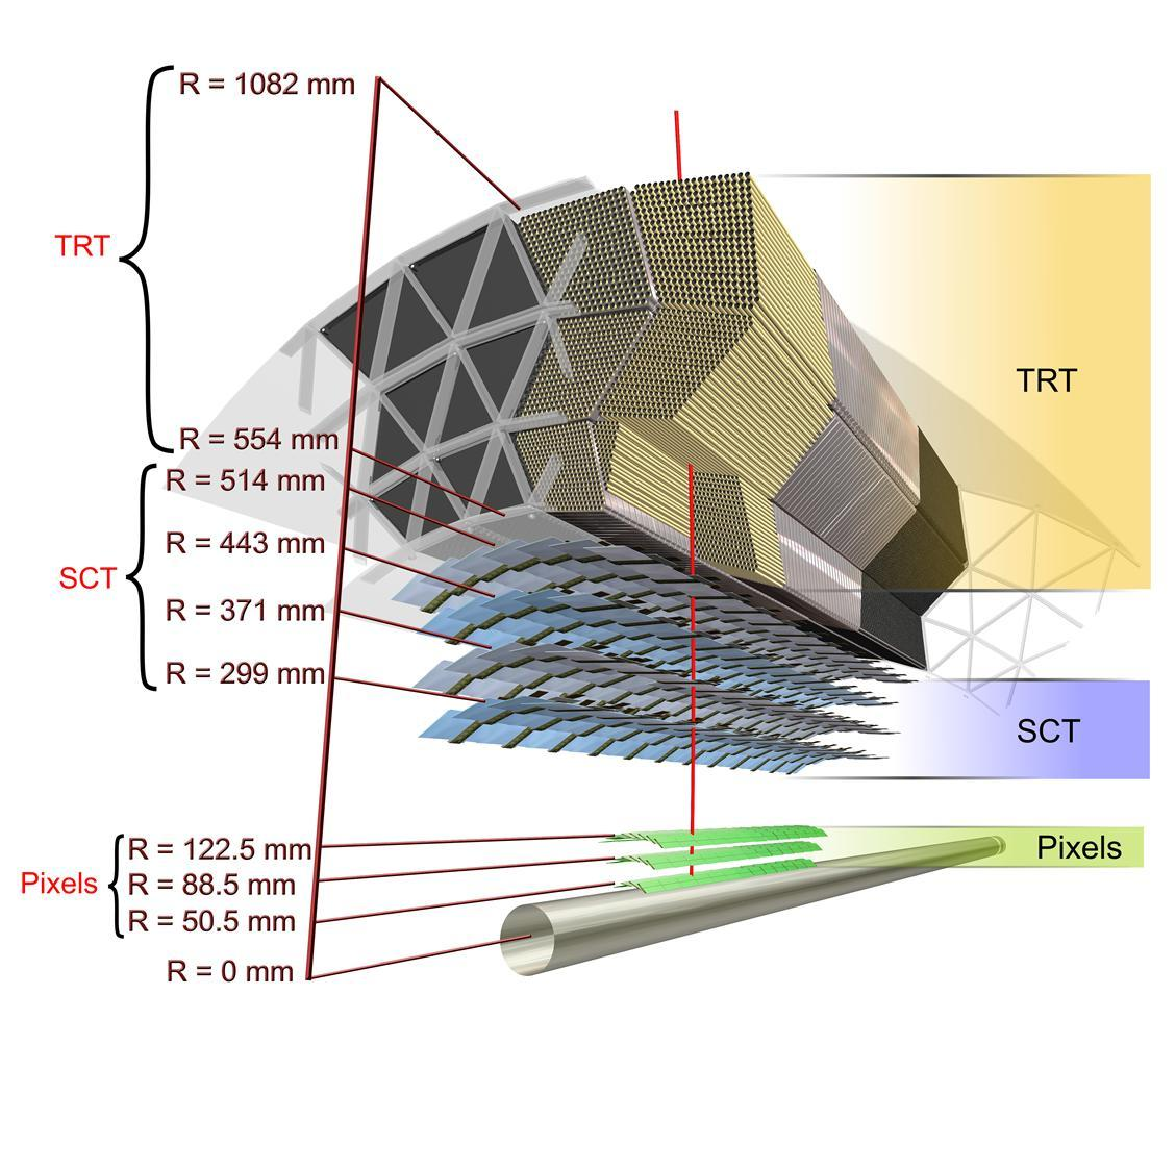
\includegraphics[width=0.6\textwidth]{detector_interno}
  \caption{Esquema del detector interno mostrando la traza de una partícula
    cargada de $\pt = 10\gev$ atravesándolo. La trayectoria atraviesa el
    tubo del haz de berilio, las tres capas del detector de píxeles de silicio (Pixels),
    las cuatro capas dobles de sensores semiconductores (SCT), y
    aproximadamente 36 tubos contenidos en los módulos del detector por radiación
  de transición (TRT).}\label{fig:detector_interno}

\end{figure}

\subsubsection{Detector de Píxeles}

Más cerca del punto de interacción se encuentra el detector de píxeles
\cite{Wermes:381263}, cuyo objetivo principal consiste en la medición de la
posición de trazas de partículas cargadas con la más alta precisión posible y es
de vital importancia para la reconstrucción de los vértices primarios y
secundarios. El principio de detección para partículas cargadas es la medida de
la deposición de la carga inducida en una capa de silicio por ionización.
Se compone de tres capas en la region \emph{barrel} (a 4, 10 y 13 cm del tubo
del haz) y tres discos en cada \emph{end-cap}.
La primer capa, conocida como capa-$B$, está ubicada a $\unit[50.5]{mm}$ del
punto de interacción, permitiendo obtener una resolución óptima del parámetro de impacto.
El sistema contiene en total 80 millones de sensores electrónicos, capaces de
resolver la posición de las partículas mejor que $\unit[14]{\mu m}$.


\subsubsection{Detector Semiconductor de Trazas (SCT)}

Por fuera del detector de píxeles se encuentra el detector semiconductor de
trazas (SCT) que consta de ocho capas de detectores de micro bandas de silicio
que provee puntos de alta precisión en las coordenadas (R$\phi$,z).
La
resolución espacial es de 16 $\mu$m en R$\phi$ y de 580 $\mu$m en z y tiene 6.2
millones de canales. Las trazas pueden distinguirse si están separadas más de
$\sim$200 $ \mu$m. El SCT cubre el rango de pseudorapidez de $|\eta|<$2.5.


\subsubsection{Detector de Radiación de Transición (TRT)}

La parte más externa del detector de trazas es el detector de radiación de
transición (TRT). Este detector está basado en el uso de detectores tubos que
pueden operar a alta frecuencia de eventos gracias a su pequeño diámetro ($\unit[4]{mm}$) y
la aislación de sus hilos centrales en volúmenes de gas individuales.

El TRT además de detectar el pasaje de partículas cargadas, detecta la radiación
de transición que permite distinguir entre partículas cargadas pesadas y
livianas. La separación entre señales de trazas y de radiación por transición se
hace analizando tubo por tubo impactos de alto umbral e impactos de baja señal.
El largo de los tubos varía segun la zona del detector, llegando hasta los 144
cm en la zona central. El \emph{barrel} contiene 50000 tubos y las
\emph{end-caps} contienen 320000 tubos orientados radialmente. El número total
de canales es de 420000 y la resolución espacial es de $\unit[0.17]{mm}$.


\subsection{Calorímetros}

Una vista de los calorímetros de ATLAS puede verse en la \cref{fig:calorimetros}.
Consiste en un calorímetro electromagnético cubriendo la región de pseudorapidez
$|\eta| < 3.2$, un calorímetro hadrónico en la sección \emph{barrel} cubriendo
la región $|\eta| < 3.2$, calorímetro hadrónicos en las \emph{end-cap} cubriendo
la región $1.5 < |\eta| < 3.2$, y calorímetros \emph{forward} cubriendo $3.1 < |\eta| < 4.9$.


\subsubsection{Calorímetro electromagnético}

\begin{figure}[!p]
  \centering

  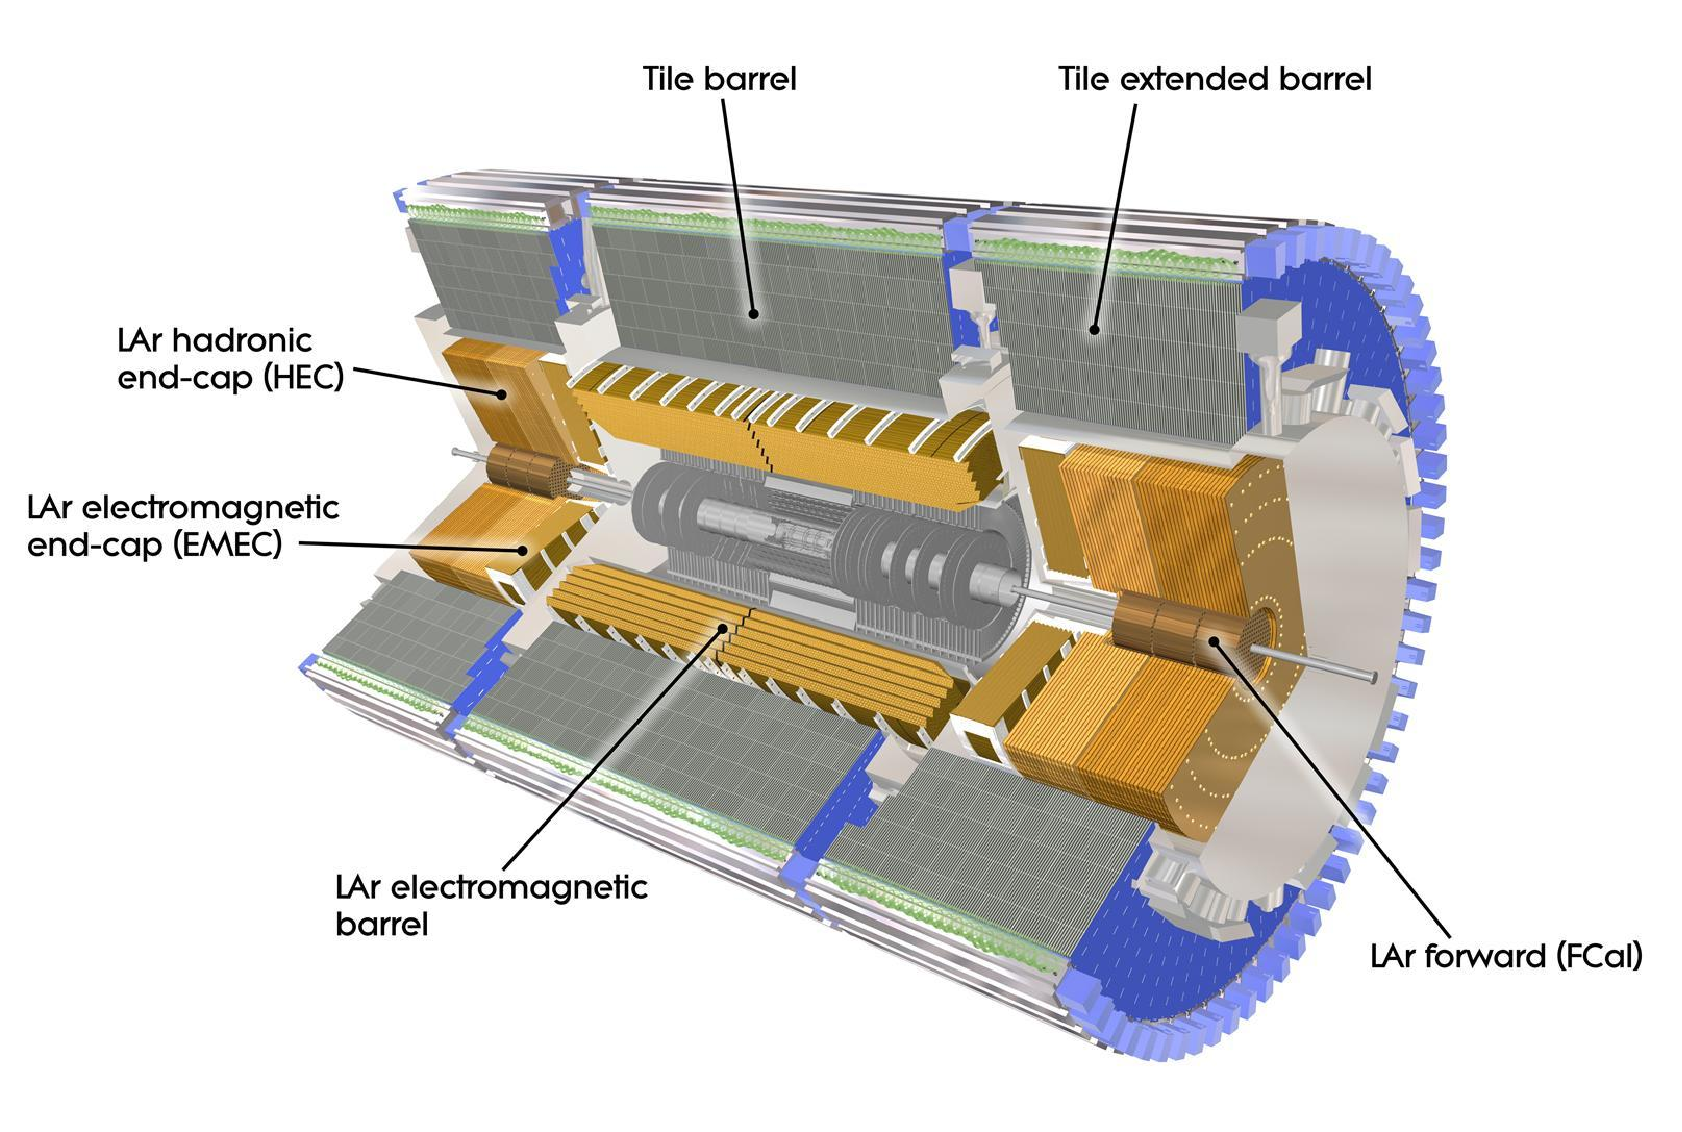
\includegraphics[width=0.9\textwidth]{calorimetros}

  \caption{Sistema de calorímetros del detector de ATLAS}
  \label{fig:calorimetros}

\end{figure}

El calorímetro electromagnético \cite{caloemTDR} se divide en una parte central
($|\eta|<$1.475) y los \emph{end-caps} (1.375$<|\eta|<$3.2). La parte central
está compuesto por dos mitades, separadas por una
distancia pequeña ($\unit[6]{mm}$) a $z = 0$. Las tapas del calorímetro están divididas en
dos ruedas coaxiales, una rueda externa cubriendo la región 1.375$<|\eta|<$2.5 y
una parte interna que cubre la región 2.5$<|\eta|<$3.2.

El calorímetro electromagnético es un detector de muestreo de argón líquido
(LAr) con electrodos de kapton en forma de acordeón y planchas absorbentes de
plomo. El espesor total del calorímetro electromagnetico es $>24 X_0$ en el
barril y $>26 X_0$ en las tapas, donde $X_0$ es la longitud de radiación.

En la región dedicada a los estudios de física de precisión ($|\eta|<$2.5) el
calorímetro electromagnético está segmentado en tres secciones longitudinales.

La sección de las bandas (\emph{strips}) que tiene un espesor constante de
$\sim 6 X_0$ en función de $\eta$, está equipado con bandas finas de $\unit[4]{mm}$ de
largo en la dirección $\eta$. Esta sección actúa como un detector de pre-cascada
aumentando la capacidad de identificación de partículas,
(como por ejemplo la distinción entre $\gamma$ y $\pi_0$ o entre electrón y
$\pi^\pm$) y dando una precisa medición de la posición en $\eta$.
La sección del medio está segmentada transversalmente en torres cuadradas de
$\Delta \phi \times \Delta \eta = 0.025 \times 0.025$ ($4 \times \unit[4]{cm^2}$ en
$\eta=0$). El espesor total del detector hasta el final de la sección del medio
es $\sim 24 X_0$.
La sección más externa tiene una granularidad de
$\Delta\phi\times\Delta\eta = 0.025 \times 0.05$ y su espesor varía entre 2 y 12
$X_0$.


\subsubsection{Calorímetro hadrónico}

El calorímetro hadrónico de ATLAS \cite{calohadTDR} cubre el rango $|\eta|<$4.9
usando diferentes materiales.
La parte del \emph{barrel} de este sistema consiste en un calorímetro de muestreo que
utiliza acero como absorbente y tejas centelladoras como material activo. Las
tejas están ubicadas radialmente y apiladas en profundidad.

La estructura es periódica en $z$. Las tejas tienen un espesor de $\unit[3]{mm}$ y el
espesor de las placas de acero en un período es de $\unit[14]{mm}$.
El calorímetro de tejas se extiende radialmente desde un radio interno de $\unit[2.28]{m}$
hasta un radio externo de $\unit[4.25]{m}$.

En la región de \emph{end-caps}, el calorímetro hadrónico consiste en dos ruedas de
$\unit[2.3]{m}$ de radio, perpendiculares al tubo del haz, hechas con placas de cobre y
tungsteno como material absorbente y argón líquido como material activo. Estos
detectores extienden la aceptancia del calorímetro de ATLAS hasta prácticamente
cubrir el ángulo sólido del punto de colisión.


\subsection{Espectrómetro de muones}
\label{sec:espectrometro_muones}

Los muones de alto {\pt} generados en el punto de interacción tienen un altísimo
poder de penetración y son poco interactuantes. Por ello el espectrómetro de
muones \cite{muonTDR} se encuentra situado en la parte más exterior del detector
ATLAS, alrededor del sistema de imanes de toroides, y está diseñado para obtener
mediciones de alta precisión de posición e impulso de muones de alto \pt.
Este es el subdetector más grande y el que le da a ATLAS su tamaño.

%% \begin{figure}[!htb]
%%   \centering
%%   \includegraphics[width=0.7\textwidth]{figures/}
%%   \caption{Espectrómetro de muones del detector de ATLAS}\label{fig:especmuones}
%% \end{figure}

%% La \cref{fig:especmuones} muestra un esquema del espectrómetro de muones
%% de ATLAS.

La región del barril está compuesta por tres capas concéntricas de cámaras de
\emph{trigger} y de cámaras de precisión posicionadas a 5m, 7.5m y 10m del tubo del
LHC, cubriendo la región $|\eta|<1$. Las regiones de las tapas están compuestas
por cuatro capas de cámaras de \emph{trigger} y cámaras de precisión a $|z|$= 7.4m,
10.8m, 14m y 21.5m cubriendo el rango de 1.0$<|\eta|<$2.7. Hay una pequeña
brecha en $|z|=0$ que permite el acceso de los servicios al ID.

El espectrómetro de muones es el subdetector más grande de ATLAS, construido
dentro y alrededor de los imanes toroidales. Los muones son altamente penetrantes
y son las únicas partículas (excepto las invisibles que no interactúan) que llegan
a el sistema de muones. Los muones pierden parte de su energía mientras penetran
las capas internas de ATLAS antes de llegar al espectrómetro de muones. La perdida
de energía tiene que ser tenida en cuenta utilizando los depósitos de energía
en los calorímetros.

%% The muon system is exposed to challenging background conditions. Final state
%% particles undergoing secondary interactions in the detector, shielding or surround-
%% ing machine material, result in a large number of particles, mainly photons and
%% neutrons with energy of order ∼ 1 MeV, penetrating the muon system. The muon
%% spectrometer is designed to cope with these high rates of particle flux. Cosmic ray
%% event data was used to measure the muon reconstruction efficiency and the momen-
%% tum resolution of the muon spectrometer [59]. For muons with transverse momenta
%% of ∼ 100 GeV the momentum resolution is at its best, with an expected fractional
%% resolution of ∼ 2 %. At p T ∼ 1 TeV this resolution decreases to ∼ 10 %, and below
%% 100 GeV the resolution also drops off as an increasing fraction of the muon energy
%% is lost traversing the detector material downstream.

%%El sistema de muones incluye
%% The muon system includes a separate trigger designed to identify events contain-
%% ing highly energetic muons, which are interesting for many new physics searches.
%% The muon trigger has coverage up to |η| < 2.4, with the full range of the muon
%% system being |η| < 2.7. Three concentric cylinders surrounding the calorimeters
%% at radii of 5 m, 7.5 m and 10 m comprise the muon system in the barrel. Wheels
%% are placed at distances of approximately 7.4 m, 10.8 m, 14 m and 21.5 m from the
%% interaction point, constituting the muon system in the end-caps. A total of four
%% different technologies are incorporated into the muon system to fulfil the triggering
%% and precision physics requirements. The Monitored Drift Tubes (MDTs) and Cath-
%% ode Strip Chambers (CSCs) provide precision energy measurements and tracking,
%% with the Resistive Plate Chambers (RPCs) and Thin Gap Chambers (TGCs) be-
%% ing responsible for triggering. A particular challenge for the muon trigger system
%% is the ability to maintain a stable p T resolution for the full |η| < 2.4, since the
%% momentum, p, of a muon of a given p T increases as a function of η. This demands
%% increased granularity in the more forward regions of the muon spectrometer so as to
%% ensure a momentum resolution consistent with the barrel. To achieve this different
%% technologies are used in the barrel and end-cap regions of the muon system.
%% The MDTs are gas filled (Ar, CO 2 ) aluminium tubes of diameter ∼ 30 mm with
%% tungsten wires immersed within. When a muon traverses these tubes the gas is
%% ionised and the resulting electrons collect on the tungsten. The MDTs are found in
%% both the barrel and the end-caps, and provide precision position and momentum
%% measurements over the full |η| < 2.7 range of the muon system. A typical MDT
%% chamber consists of two multi-layers of drift tubes, which are separated by spacer
%% bars made of aluminium. Each of these multi-layers contains four layers of tubes
%% in the barrel, or three in the outer regions of the muon system. This means that a
%% muon penetrating the MDTs will on average pass through 20 individual tubes.
%% The safe operational counting rate per unit area for the MDTs is exceeded in
%% the forward regions of the muon system. Cathode strip chambers, with a quicker
%% response time and double the resolution, are used in this region. The CSCs cover the
%% range 2.0 < |η| < 2.7 and are used in the innermost part of the muon system in the
%% end-caps. They are multi-wire proportional chambers containing multiple closely
%% spaced anode wires surrounded by gas (Ar, CO 2 , CF 4 ), with cathode strips running
%% perpendicular to the wires. This orthogonal layout allows the charge distribution
%% to be measured in both directions normal to the beam axis. The CSC system itself
%% is segmented in φ, resulting in eight chambers in each of the two disks. With four
%% CSC layers in each chamber, the average number of measurements per track is
%% considerably less than in the MDTs.
%% The RPCs make up the barrel part (|η| < 1.05) of the dedicated trigger system.
%% Two resistive plates are separated by 2 mm of gas (C 2 H 2 F 4 , Iso-C 4 H 10 , SF 6 ), which
%% may be ionised by a muon passing through, causing a cascade of electrons towards
%% the anode. These chambers are made simpler in construction due to the absence
%% of any wires within, and this feature also makes them less sensitive to any small
%% deviations in positioning (e.g. wire sag). There are three cylindrical trigger layers
%% in the barrel, and each layer contains two RPCs. As such, a muon in the barrel will
%% deliver six hits in the RPCs. The RPCs are able to provide adequate triggering for
%% the barrel region.
%% In addition to the increased demands on granularity, the forward region suffers
%% from radiation levels up to 10 times those in central regions. This further compli-
%% cates the already challenging environment in the end-caps. The TGCs are used to
%% trigger on muon tracks in the end-caps (1.05 < |η| < 2.4). They are multi-wire
%% proportional chambers working similarly to the CSCs, but in this case in order to
%% satisfy the higher granularity requirements the gap between the wire and cathode
%% is smaller than the wire-wire spacing. They exist in two concentric rings, one inner
%% ring containing two TGC layers and one outer ring containing seven. These layers
%% are segmented radially, are tailored to provide excellent time resolution and are able
%% to cope with high particle flux rates. Both the TGCs and RPCs are designed to
%% deliver signals over a time spread of less than 25 ns. This way the bunch crossing
%% responsible for the muon triggering the chamber can be identified with an efficiency
%% of > 99 %.


%---------
% Trigger
%---------
\section{El sistema de \emph{trigger}}

La parte central del sistema de adquisición de datos de ATLAS es el
<<\emph{trigger}>>. El sistema de \emph{trigger} puede ser pensado como un filtro que
selecciona, del gran número de colisiones que tienen lugar en el experimento,
los eventos que serán almacenadas para su posterior procesamiento y análisis.

El LHC esta disenado para proveer colisionesión $pp$ de $\mathcal{O}(1)$ GHz,
considerando una frecuencia de cruce de haces de $\unit[40]{MHz}$ y $\sim$ 23
interacciones por cruce. Dado que la mayoría de los eventos no son de interés
para los análisis de fisica, y también debido a las limitaciones de
almacenamiento y de poder de cómputo, el flujo de datos incidente debe ser
reducido al máximo permitido para su almacenamiento permanente ($\sim 400$ Hz)
\cite{Aad:2012xs}.
Esta reducción se logra mediante una rápida y eficiente preselección de eventos,
conocida como \emph{trigger}.

Esencialmente, el sistema de \emph{trigger} de ATLAS \cite{atlas} consiste en
una selección de eventos basada en tres niveles: Nivel 1 (L1), Nivel 2 (L2) y
Filtro de eventos (EF), donde los dos últimos conforman el \emph{High Level
  Trigger} (HLT). Cada nivel permite analizar los eventos con mayor detalle,
aumentando la precisión de los criterios de selección y la complejidad de los
algoritmos utilizados. El sistema de adquisición de datos transfiere y
almacena los datos seleccionados por el \emph{trigger}.

El L1 se encarga de la selección inicial, reduciendo la frecuencia de eventos
que pasan al siguiente nivel a $\sim 75$ kHz. Debido al tamaño limitado de las
memorias temporales donde se guardan los datos de cada subdetector y al
considerable tiempo de vuelo de las partículas hasta el espectrómetro de muones,
la decisión debe tomarse en una escala de tiempo muy limitada ($\unit[2.5]{\mu
  s}$). El L1 esta basado en hardware y selecciona objetos de alto {\pt}
construidos a partir de la información de varios subdetectores. Los muones son
identificados en las cámaras de trigger descriptas en la
\cref{sec:espectrometro_muones}, mientras que la información de los
calorímetros, con una resolución reducida, se utiliza para identificar
candidatos a electrones, fotones, jets y taus decayendo hadrónicamente. La
posición de cada objeto encontrado define una <<región de interés>> (RoI) en
un evento potencialmente interesante, que se extiende como un cono desde el
punto de interacción a lo largo del detector.

En el calorímetro, el L1 se basa en las señales analógicas obtenidas en cada
torre del trigger, es decir en la suma de celdas en una ventana $\Delta \eta
\times \Delta \phi = 0.1 \times 0.1$, definida separadamente para el calorímetro
electromagnético y hadrónico. La aceptancia geométrica del L1 está ligada al
diseño del detector, donde las medidas de precisión en los calorímetros y la
cobertura del detector interno están limitadas a la región $\abseta < 2.5$. El
trigger de fotones, electrones, muones y taus debe asegurar la cobertura en esta
región. En el caso del trigger de jets, las torres del \emph{trigger} se
extienden hasta $\abseta < 3.2$, mientras que para el cálculo de la energía
transversa total (faltante) se utiliza todo el sistema calorimétrico (es decir,
$\abseta < 4.9$). Los resultados de los subsistemas del trigger son procesados
en el \emph{Central Trigger Processor}, en donde se aplica una serie de
selecciones definidas como una combinación de criterios individuales, que pueden
ser ajustados según la luminosidad y los requerimientos físicos particulares de
cada toma de datos. Las distintas configuraciones (\emph{items}) están
disponibles en el L1, donde se programa el tipo de RoI (EM, TAU, JET, etc.) y
los umbrales de energía total y de aislamiento requeridos en cada caso. Por
ejemplo, el item L1EM14 acepta eventos donde al menos un (dos) cluster(s) en el
calorímetro electromagnético posee(n) $\et \geq 14 \GeV$.

El segundo nivel del trigger (L2) se centra únicamente en las RoIs donde el L1
encontró actividad, combinando información de todos los subdetectores dentro de
cada una ($\sim 2$ \% de la cobertura total del detector). El L2 consiste de una
serie de algoritmos de reconstrucción y selección especializados, dise\~nados
para reducir la frecuencia de eventos hasta aproximadamente 1 kHz. Estos
algoritmos están implementados en clusters de procesamiento dedicados
que analizan cada evento dentro de un tiempo de latencia medio de $\sim
\unit[40]{ms}$. El menor flujo de información en este nivel del trigger permite
calcular las variables calorimétricas con mayor precisión y hacer uso de la
información de las trazas reconstruidas, haciendo posible la distinción entre
fotones y electrones, y el rechazo de fondo proveniente en su mayoría de jets.
En general, si bien la selección se basa en las mismas variables que la
identificación \emph{offline} descripta en la \cref{sec:obj_photons} (sobre las características de
las lluvias electromagnéticas), los valores de corte en cada variable son
relajados (o a lo sumo igualados) respecto a la selección offline, para evitar
el rechazo prematuro de candidatos que satisfacen los criterios de identificación
durante el análisis final. La última etapa de la selección del trigger se lleva
a cabo en el EF, que reduce la frecuencia de eventos a $\sim \unit[400]{Hz}$.
En este nivel se tiene acceso a toda
la información del evento en los distintos subdetectores de ATLAS, con la máxima
granularidad e incluyendo detalles sobre la calibración de energía de los
calor metros, la alineación de los subdetectores y el mapa de campo magnético. El
tiempo de latencia relativamente largo disponible para tomar la decisión final
sobre el evento ($\avg{t} \sim \unit[4]{s}$) permite la reconstrucción completa
del mismo, y el refinamiento de las variables y criterios de selección al nivel
de aquellos implementados en el análisis offline. Los eventos aceptados por el
EF son finalmente grabados a disco y distribuidos, accesibles \emph{offline} para todos
los análisis subsecuentes.

Al igual que en el L1, en cada nivel del HLT se configuran ciertos
criterios según el tipo y multiplicidad de la partícula que se busca en el
evento, y el conjunto de cortes de identificación aplicados. La nomenclatura
adoptada como convención en el trigger de ATLAS tiene la forma general
\texttt{L\_ipX\_Y}, donde \texttt{L} es el nivel del trigger (L2,EF), \texttt{i}
la multiplicidad, \texttt{p} la partícula de interés (por ejemplo
\texttt{g} = fotón, \texttt{e} = electrón), \texttt{X} el {\pt} mínimo requerido e
\texttt{Y} el tipo de identificación aplicada (loose, tight, etc.). Los
distintos criterios del L2/EF y su item asociado en el L1 definen en conjunto
una de las \emph{cadenas} del trigger, que toman el nombre de la signature del
HLT (es decir,  \texttt{ipX\_Y} según la convención anterior) y conforman el \emph{menu} final
del trigger.

Para cada item del trigger se puede asignar además
un factor de escala o prescale (PS), que define la frecuencia con la que un dado
item es evaluado por el trigger (es decir solo en uno de cada PS eventos).
Se habla de una cadena de trigger \emph{unprescaled} si su factor de escala es
$\text{PS} = 1$ en cada nivel, es decir, es evaluada en todos los eventos. La asignación de estos
factores se hace incluso dinámicamente durante una toma de datos, para tener en
cuenta el descenso de la luminosidad instantánea con el tiempo y mantener la
tasa de procesamiento aproximadamente constante.



\section{Modelo computacional y distribución de datos}

El modelo computacional de ATLAS esta diseñado para permitir a todos los
miembros de la colaboración un acceso ágil, directo y distribuido a la gran
cantidad de datos recolectados por el detector ($\sim \text{PB}/\text{a\~no}$),
así como a las diversas simulaciones MC. El modelo se basa en la tecnología
GRID, compartiendo el poder de procesamiento y la capacidad de almacenamiento
disponibles en distintos centros de cómputo asociados alrededor del mundo.

El software de ATLAS se desarrolla dentro un entorno C++ común llamado
\textsc{Athena} \cite{CompuTDR,Lenzi:1214931,Calafiura:865624}, basado en el
proyecto GAUDI \cite{Gaudi}. Todo el procesamiento de los datos en ATLAS se
realiza dentro de este entorno, incluyendo la implementación y configuración del
HLT, la simulación de la respuesta del detector, la generación de las muestras
MC de los distintos procesos físicos, y la reconstrucción y análisis de los
datos. Los eventos aceptados por el trigger deben ser procesados para reducir su
tamaño y ser utilizados para los análisis offline. A la salida del HLT, los
eventos son almacenados como RDOs (\emph{Raw Data Objects}). Luego de aplicar
los algoritmos de reconstrucción y calibración, las colecciones de los distintos
objetos físicos obtenidas (fotones, electrones, etc.) son almacenadas en formato
ESD (\emph{Event Summary Data}) y AOD (\emph{Analysis Data Object}), una versión
reducida del primero ($\sim 100$ kB/evento). A partir de las ESD/AOD, se ha
definido un formato de datos significativamente más pequeño (10-15 kB/evento)
conocido como D3PD (\emph{Derived Physics Data}), sobre el que se realiza el
análisis final. Las \emph{D3PD} son ntuplas almacenadas en un formato de archivo
accesibles vía el entorno de análisis de datos ROOT \cite{Brun199781}, que
contienen un conjunto de variables para diferentes objetos físicos, según las
necesidades de cada grupo de análisis dentro de ATLAS. Para el análisis de esta
tesis, se utilizaron las D3PD definidas y producidas en forma centralizada por
el grupo de SUSY. La misma cadena de reconstrucción y distribución se aplica a
las simulaciones Monte Carlo, a fin de conservar un modelo de análisis único y
garantizar la consistencia en la comparación de estas con los datos
experimentales.

%% 2 ATLAS \emph{offline} Software Overview
%% The ATLAS software framework, Athena [3], uses Python
%% as an object-oriented scripting and interpreter language
%% to configure and load C++ algorithms and objects.
%% Rather than develop an entirely new high-energy physics
%% data processing infrastructure, ATLAS adopted the Gaudi
%% framework [6, 7], originally developed for LHCb and written
%% in C++. Gaudi was created as a flexible framework to
%% support a variety of applications through base classes and
%% basic functionality. As much as possible, the infrastructure
%% relies on the CLHEP common libraries [8], which include
%% utility classes particularly designed for use in high-energy
%% physics software (e.g. vectors and rotations).
%% Athena releases are divided into major projects by
%% functionality [9], and all of the ATLAS simulation software
%% (including event generation and digitization) resides
%% in a single project. The dependencies of the “simulation”
%% project are the “core” project, which includes the Athena
%% framework, the “conditions” and “detector description”
%% projects, which include all code necessary for the description
%% of the ATLAS detector, and the “event” project,
%% which includes descriptions of persistent objects. The number
%% of lines of code by software language for the simulation
%% project are summarized in Table 1, as calculated using
%% cloc [10] in Athena release 14.4. Lines of code in the upstream
%% Athena projects, excluding external dependenccies
%% like Gaudi and CLHEP, are summarized in Table 2.



\section{Datos de colisiones $pp$ a $\sqrt{s} = 8$ \tev}

Durante la operación del detector ATLAS, cada toma de datos (\emph{Run}) durante
un haz estable provisto por el LHC, es dividida en bloques de luminosidad
(\emph{LB}) de aproximadamente dos minutos, dentro de los cuales la luminosidad
instantánea es prácticamente constante, y en el que se espera que las
condiciones del haz sean estables. Producto de la complejidad del experimento y
de las demandantes condiciones de funcionamiento del LHC, se pueden observar
ocasionalmente ciertas ineficiencias en los diversos subdetectores y/o en la
cadena de procesamiento de los datos recolectados. Durante cada \emph{Run} los
distintos subcomponentes del detector son monitoreados y cada problema es
registrado, incluyendo que componenentes están inactivos, o si hay problemas en
la infraestructura o en el haz.

Para asegurar la calidad de los datos a ser considerados en los análisis físicos
de ATLAS, los grupos responsables de cada subdetector definen un conjunto de
criterios de calidad \cite{GRL}, con los cuales se construyen listas, llamadas
GRL (\emph{Good Runs List}), de las \emph{Runs} y los rangos de LB dentro de ellas que
son apropiados para cada tipo de análisis. Se producen de forma centralizada
para brindar listas oficiales comunes para los distintos grupos dentro de ATLAS
y son distribuidas en un formato \textsc{XML} para luego ser utilizadas durante
el análisis final. Cada análisis elije que GRL utiliza dependiendo de su
tolerancia a las fallas de los subdetectores.

El presente análisis utiliza el conjunto de eventos recolectados de las colisiones
$pp$ a una energía de centro de masa $\sqrt{s} = 8\tev$ con el detector ATLAS
durante el a\~no 2012. Estos eventos recolectados corresponden a una luminosidad
total integrada de 21.7 \ifb. Dado que en el análisis se utilizan fotones, electrones,
muones, jets y energía faltante, es imprescindible que todos los subsistemas
del detector ATLAS hayan operado en condiciones normales durante la toma
de datos. Este requerimiento adicional resulta en una reducción de los datos de
$\sim 6\%$, dejando una luminosidad total de $\int L\, dt = 20.3 \pm 0.6\, (2.8
\%) \, \ifb$\cite{lumi2012} para análisis físicos.

Otro concepto importante de la toma de datos en ATLAS es el \emph{pile-up}, el
cual ocurre cuando las partículas producidas en más de una colisión
partón-partón llegan al detector al mismo tiempo, o más generalmente que sus
señales se superponen de una forma que no puede ser separadas. Cuando los
\emph{bunches} de protones colisionan, la probabilidad de una interacción es
proporcional a la densidad de partículas, o mejor, al flujo de partículas, el
cual se expresa con la luminosidad instantánea. El número de colisiones de
partículas real que tienen lugar cuando dos \emph{bunches} se cruzan es una
variable aleatoria que sigue una distribución de Poisson. Para bajas
luminosidades, en la mayoría de los cruces de haces, no ocurre nada, pero para
luminosidades instantáneas altas, en la mayoría de los cruces se producen muchas
colisiones de partículas al mismo tiempo. Dependiendo del subdetector y el tipo
de medición, puede o no ser posible distinguir entre las partículas provenientes
de diferentes interacciones simultáneas. Esto es llamado \emph{pile-up in-time}.
En cambio, el \emph{pile-up out-of-time} incluye los efectos que se originan
cuando el tiempo que el detector necesita para volver a su estado de espera es
mayor al tiempo entre cruces de \emph{bunches}. Una medida cuantitativa del
\emph{pile-up} y la actividad en el eventos es el valor medio de interacciones
inelásticas $pp$ por cruce de \emph{bunches}, $\avg{\mu}$.

Durante el período de toma de datos del 2012, el pico de luminosidad instantánea
aumento desde $\unit[2.74 \cdot 10^{30}]{cm^{-2} s^{-1}}$ hasta
$\unit[7.61 \cdot 10^{33}]{cm^{-2} s^{-1}}$, y el número medio de interacciones por cruce
de haz varió entre 5.9 y 36.53. La distribución de la luminosidad acumulada
durante la toma de datos y del número de interacciones por colisión pude verse en
la \cref{fig:lumi}.

\begin{figure}[!p]
  \centering

  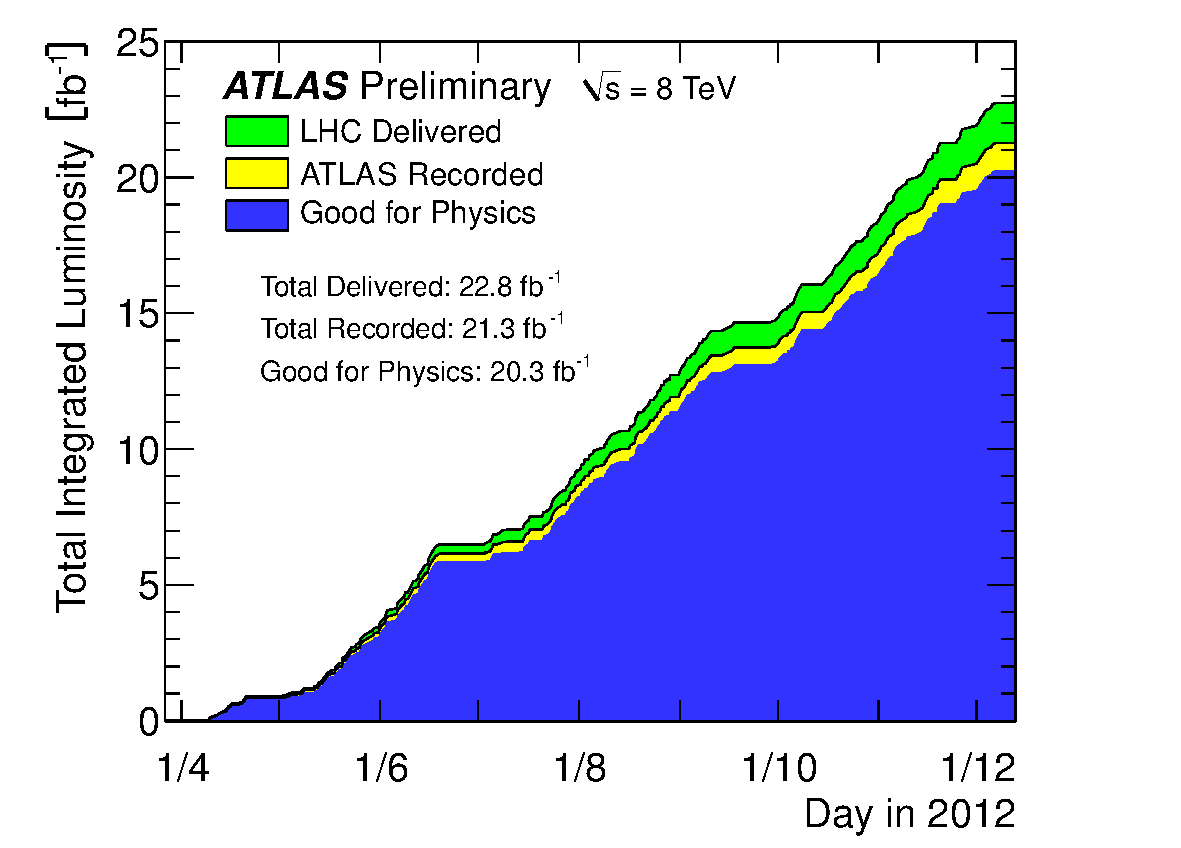
\includegraphics[width=0.49\textwidth]{intlumivstime2012DQ}
  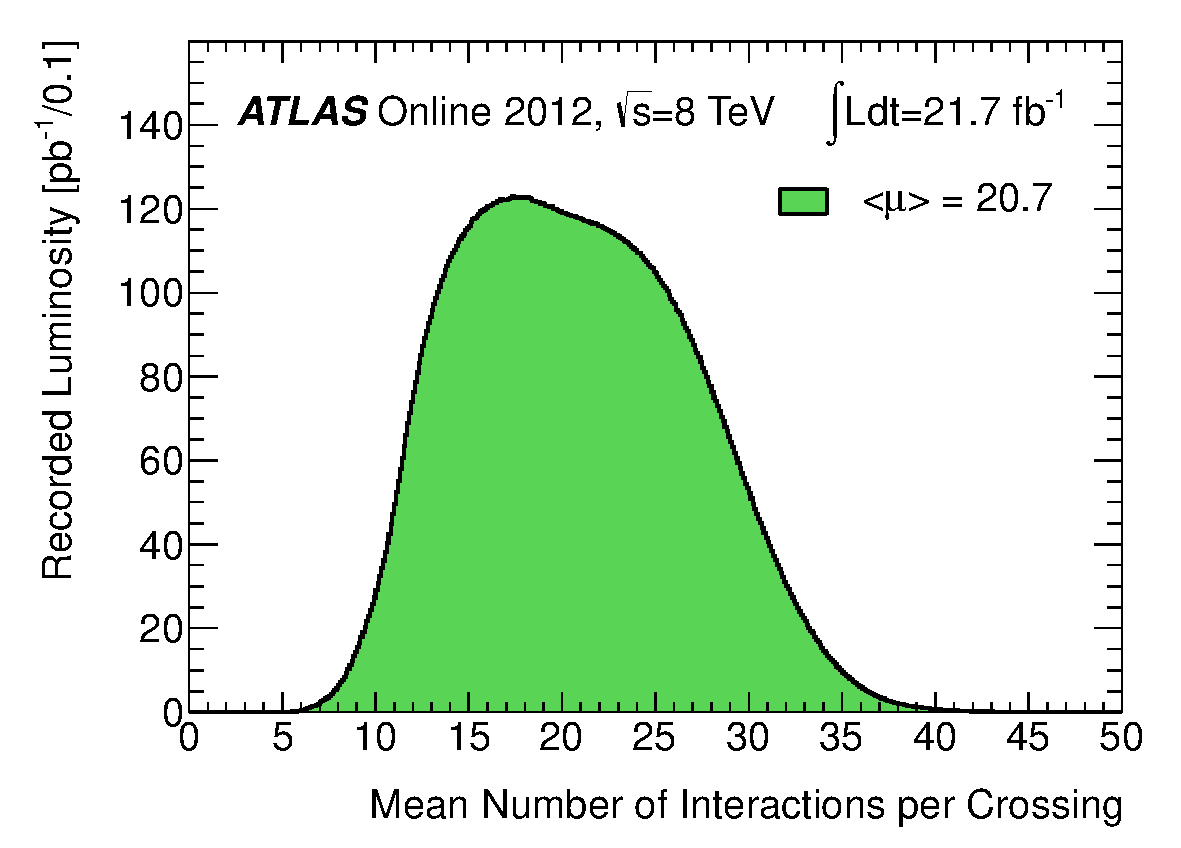
\includegraphics[width=0.49\textwidth]{mu_2012-dec}

  \caption{Izquierda: Luminosidad acumulada como función del tiempo, entregada por el LHC (verde),
    guardada por ATLAS (amarillo), y que pasa los criterios de calidad (azul),
    durante el funcionamiento del LHC con haces estables en colisiones $pp$ a $\sqrt{s}=8\tev$ durante el a\~no 2012\cite{lumiplots}.
    Derecha: Distribución del valor medio del número de interacciones por cruce
    de haz ($\mu$) durante la toma de datos en el a\~no 2012 pesado con la luminosidad.
    La luminosidad integrada y el valor medio de $\mu$ están detallados en la figura.
  }
  \label{fig:lumi}

\end{figure}
